\documentclass{article}
\usepackage{geometry}
\usepackage{graphicx}
\usepackage{amsmath}
\usepackage{algorithm}
\usepackage{algpseudocode}
\usepackage{dsfont}
\usepackage{amssymb}
\usepackage{multicol}
\usepackage{wrapfig}
\geometry{
a4paper,
right=10mm,
left=10mm,
top=10mm,
bottom=10mm,	
}

\begin{document}

\pagenumbering{gobble}

\begin{center}
\textbf{\Large HOMEWORK 3 : CS771} \\
\textit{\large Jayant Agrawal}         14282
\end{center}
\section{Problem 1- Kernel Perceptron}
\begin{figure}[h!]
\centering
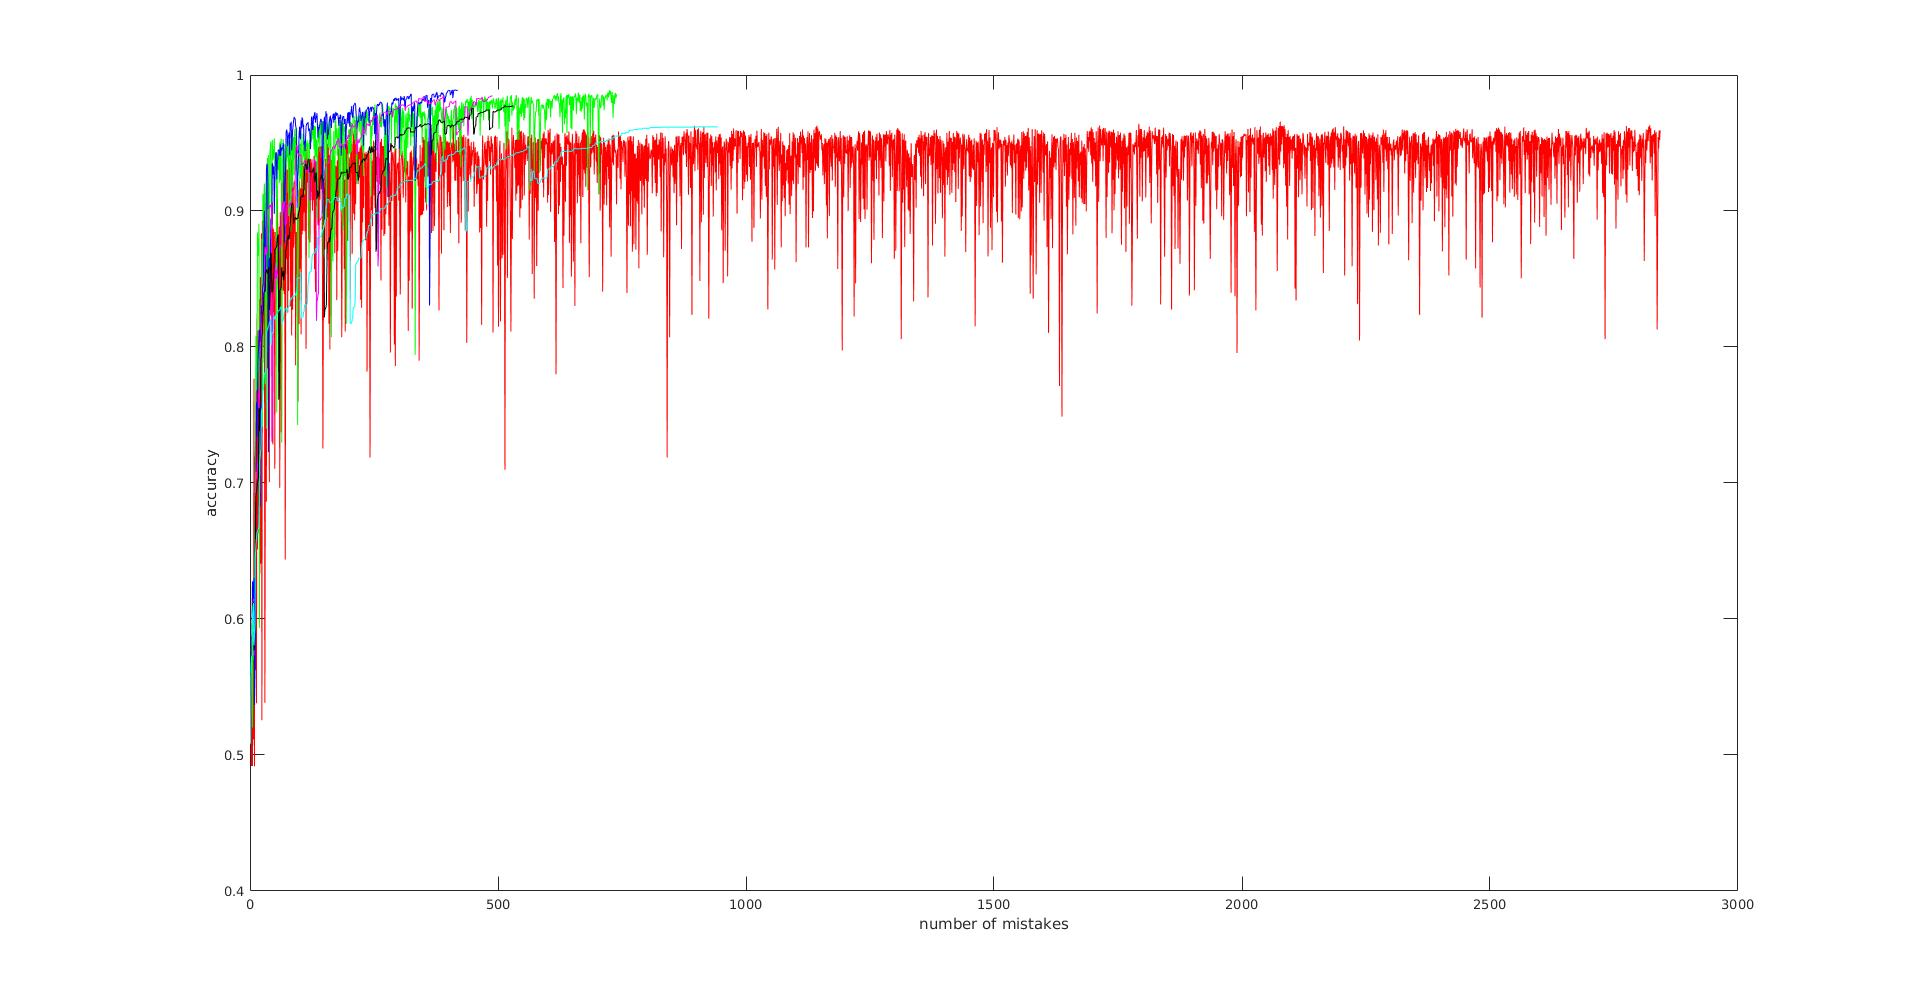
\includegraphics[width=1\columnwidth]{plot_acc.jpg}
\caption{Red = 1, Green = 2, Blue = 4, Pink = 8, Black = 10, Cyan = 20}
\label{acc}
\end{figure}
\begin{center}
\emph{Kernel with Test Accuracy: }4 (Blue)\\ 
\emph{Kernel with Minimum Mistakes: }4 (Blue) 
\end{center}

\section{Problem 2- Matrix Factorization}
\begin{figure}[h!]
\centering
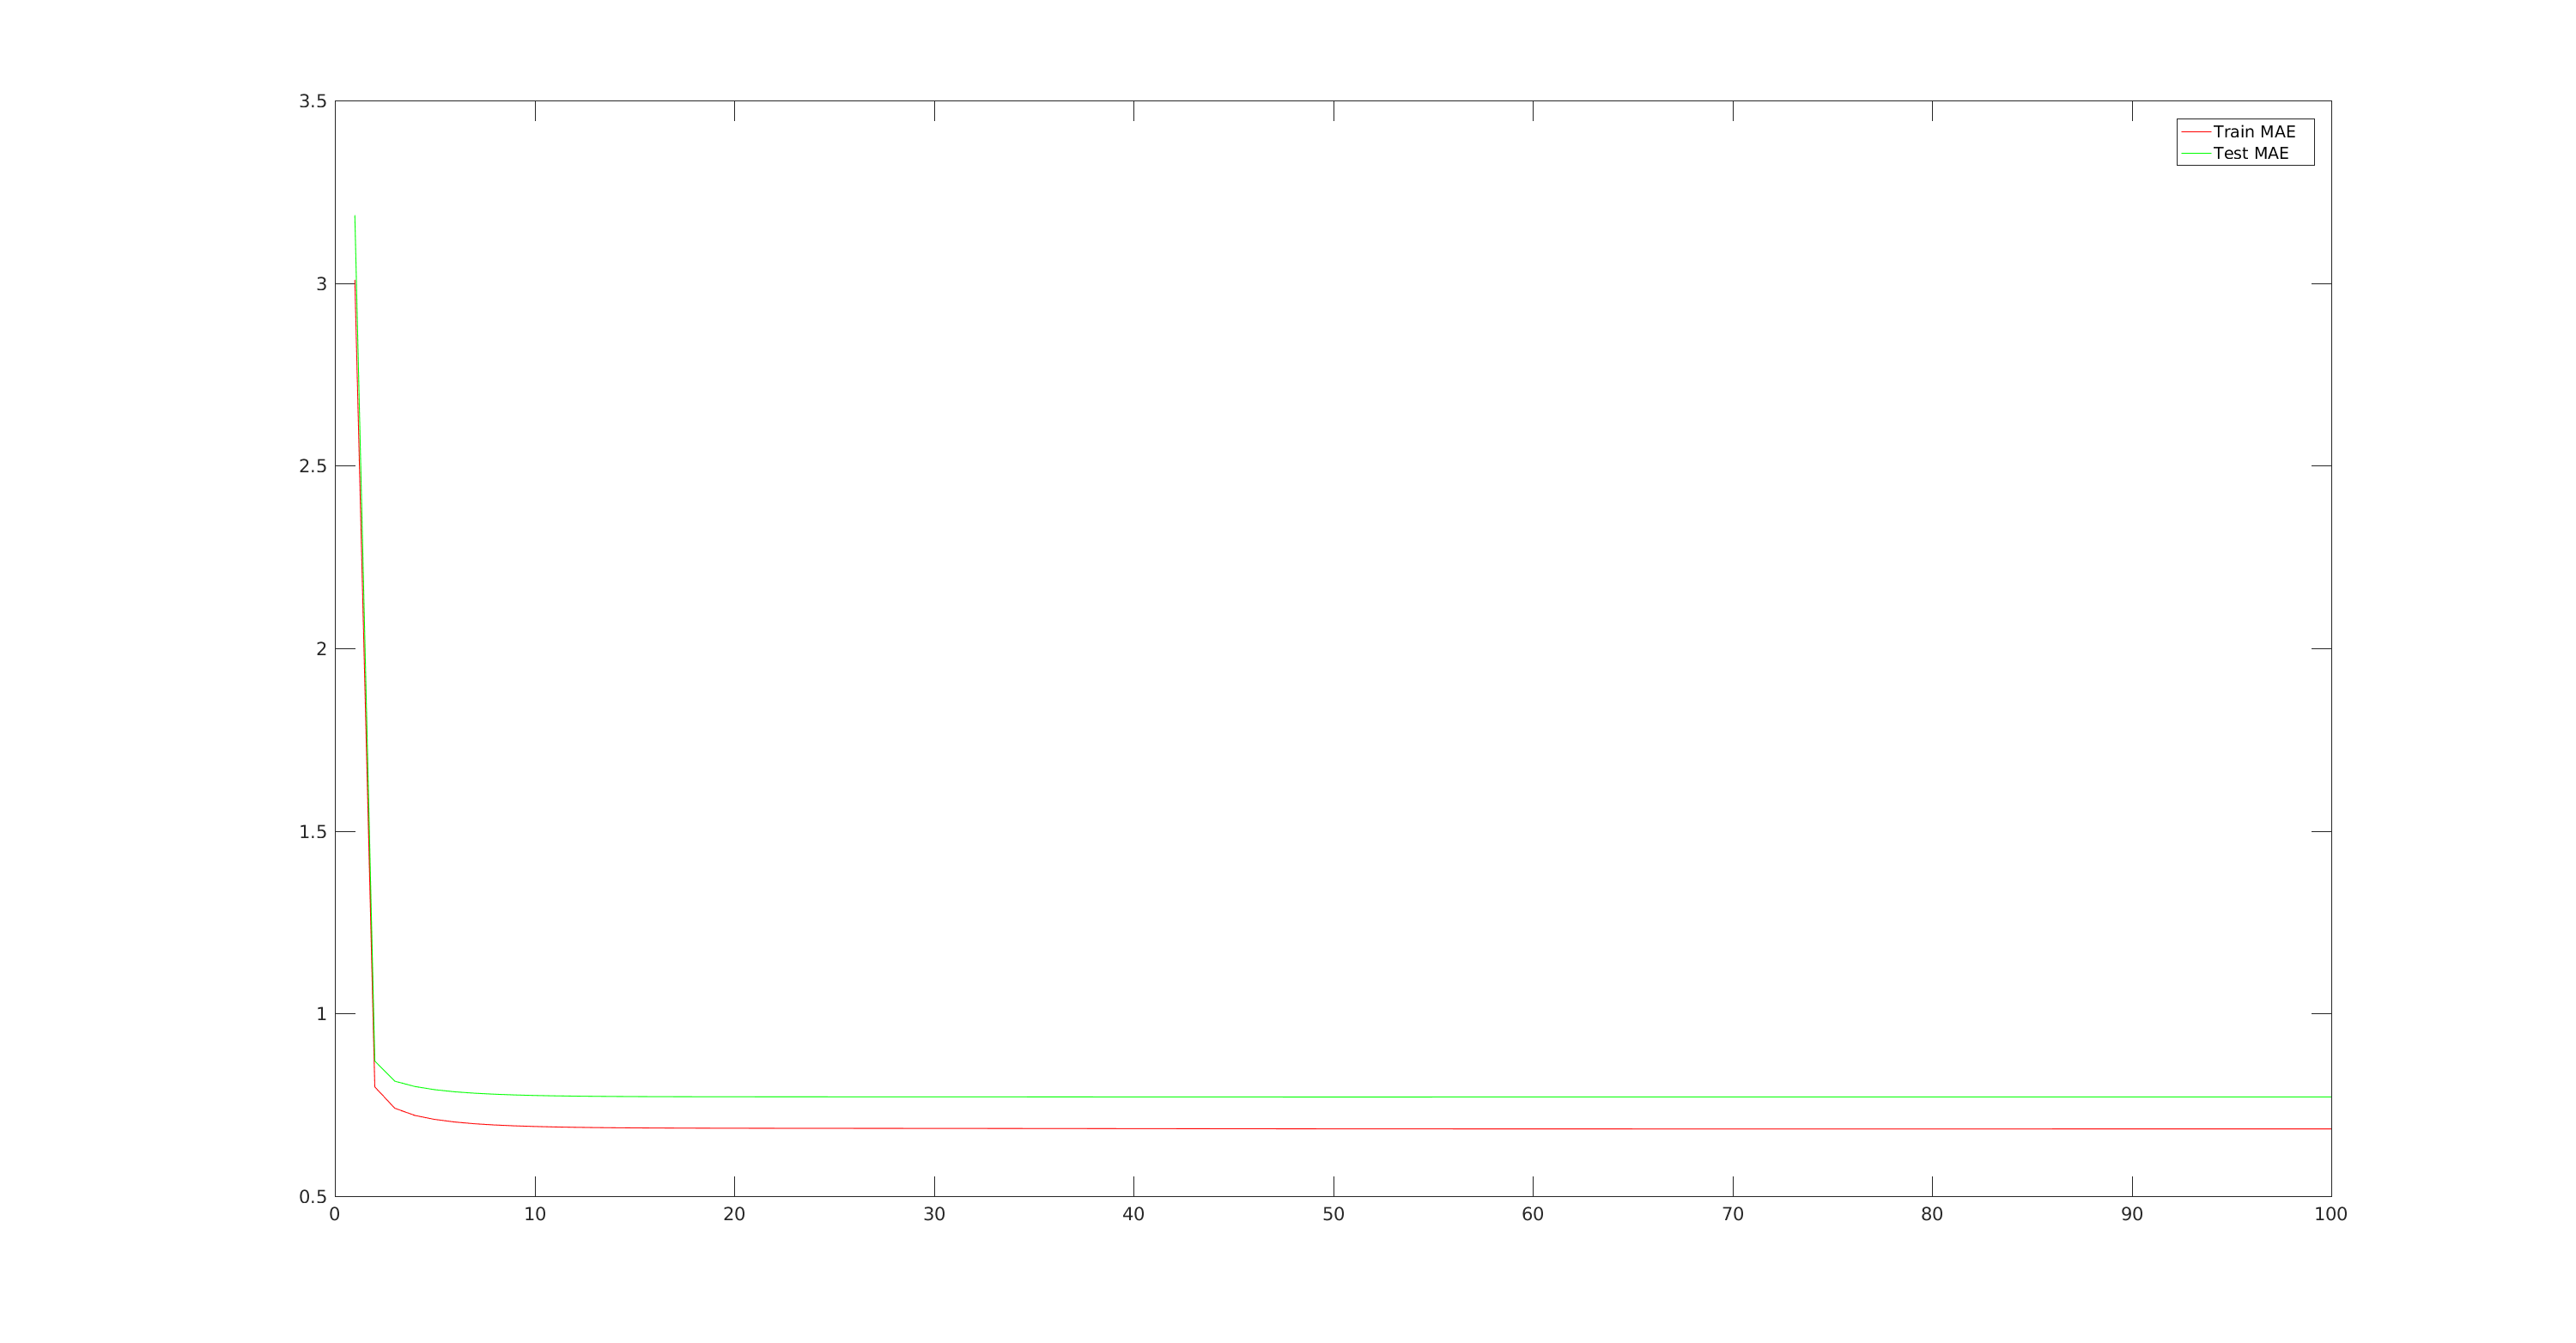
\includegraphics[width=1\columnwidth]{mae2.png}
%\caption{Red = 1, Green = 2, Blue = 4, Pink = 8, Black = 10, Cyan = 20}
\label{mae}
\end{figure}

\section{Problem 3}
\section{Problem 4}
\section{Problem 5}
\end{document}


